\chapter{Appendix}\label{chapter:Appendix}

\section{Results Data Leakage}
\sisetup{
  table-format = 1.4,    % maximal 1 Vorkommastelle, 4 Nachkommastellen
  detect-all            % übernimmt Schriftart/Fettdruck
}

% ---------- eigene Spaltentypen ----------
\newcolumntype{d}{S}     % „d“ steht für Dezimalspalte

\begin{table}[htbp]
\centering
\caption{OpenAI GPT-4o: Data Leakage (DL) based on 3 iterations}
\small                 % optional verkleinern
\setlength{\tabcolsep}{6pt} % enger packen, falls nötig
\begin{tabular}{
  l               % Model
  l               % Prompt
  | d        % Full Page (3 Spalten)
  | d d d d d     % Interaction Part (5 Spalten)
}
\toprule
\cmidrule(lr){3-3}\cmidrule(l){4-8}
\multicolumn{2}{c|}{\textbf{}} & {\bfseries Final Score} & {Size} & {Text} & {Position} & {Text Color} & {CLIP}\\
\midrule
% ---------------- Modell 1 ----------------
\multirow{4}{*}{DL Test Dataset} 
  & Naive & \bfseries 0.8917 & 0.8812 & 0.9701 & 0.8562 & 0.8451 & 0.906\\
  & Zero-Shot    & \bfseries 0.8889 & 0.866 & 0.9737 & 0.8543 & 0.8407 & 0.9098\\
  & Few-Shot   & \bfseries 0 & 0 & 0 & 0 & 0 & 0\\
  & Reasoning & \bfseries 0.8924 & 0.8819 & 0.9755 & 0.8498 & 0.8449 & 0.91\\
  & Iterative & \bfseries 0.8908 & 0.8819 & 0.9748 & 0.8475 & 0.8391 & 0.9109\\
  & Iterative Refine 1 & \bfseries 0.8878 & 0.8729 & 0.974 & 0.8469 & 0.8372 & 0.9081\\
  & Iterative Refine 2 & \bfseries 0.8887 & 0.8642 & 0.9771 & 0.8516 & 0.8439 & 0.9069\\
  & Iterative Refine 3 & \bfseries 0.8871 & 0.8497 & 0.979 & 0.8511 & 0.8483 & 0.9076\\
\midrule
% ---------------- Modell 2 ----------------
\multirow{4}{*}{Experiment Dataset}
  & Naive & \bfseries 0.8896 & 0.868 & 0.9661 & 0.8578 & 0.8456 & 0.9107\\
  & Zero-Shot    & \bfseries 0.8779 & 0.8124 & 0.9663 & 0.8558 & 0.8467 & 0.9083\\
  & Few-Shot   & \bfseries 0 & 0 & 0 & 0 & 0 & 0\\
  & Reasoning & \bfseries 0.8791 & 0.8348 & 0.9652 & 0.8549 & 0.8358 & 0.9048\\
  & Iterative & \bfseries 0.8854 & 0.8447 & 0.9694 & 0.8577 & 0.8412 & 0.914\\
  & Iterative Refine 1 & \bfseries 0.8786 & 0.8306 & 0.9677 & 0.858 & 0.8233 & 0.9131\\
  & Iterative Refine 2 & \bfseries 0.8767 & 0.8148 & 0.968 & 0.854 & 0.8315 & 0.915\\
  & Iterative Refine 3 & \bfseries 0.8731 & 0.811 & 0.9685 & 0.855 & 0.8181 & 0.9127\\
\midrule
% ---------------- weitere Modelle hier ----------------
% (dupliziere das obige Muster)
\bottomrule
\end{tabular}
\end{table}

\begin{table}[htbp]
\centering
\caption{Gemini-2.0-flash: Data Leakage (DL) based on 3 iterations}
\small                 % optional verkleinern
\setlength{\tabcolsep}{6pt} % enger packen, falls nötig
\begin{tabular}{
  l               % Model
  l               % Prompt
  | d        % Full Page (3 Spalten)
  | d d d d d     % Interaction Part (5 Spalten)
}
\toprule
\cmidrule(lr){3-3}\cmidrule(l){4-8}
\multicolumn{2}{c|}{\textbf{}} & {\bfseries Final Score} & {Size} & {Text} & {Position} & {Text Color} & {CLIP}\\
\midrule
% ---------------- Modell 1 ----------------
\multirow{4}{*}{DL Test Dataset} 
  & Naive & \bfseries 0.8801 & 0.7992 & 0.9685 & 0.8591 & 0.8251 & 0.9079\\
  & Zero-Shot    & \bfseries 0.8798 & 0.8297 & 0.977 & 0.8645 & 0.8141 & 0.9134\\
  & Few-Shot   & \bfseries 0 & 0 & 0 & 0 & 0 & 0\\
  & Reasoning & \bfseries 0.8683 & 0.799 & 0.9741 & 0.8541 & 0.8093 & 0.905\\
  & Iterative & \bfseries 0.8823 & 0.8298 & 0.9742 & 0.8624 & 0.836 & 0.9091\\
  & Iterative Refine 1 & \bfseries 0.8783 & 0.8297 & 0.9753 & 0.8616 & 0.8136 & 0.9112\\
  & Iterative Refine 2 & \bfseries 0.8874 & 0.8617 & 0.9774 & 0.871 & 0.8182 & 0.9086\\
  & Iterative Refine 3 & \bfseries 0.8899 & 0.8682 & 0.9773 & 0.8719 & 0.8224 & 0.9099\\
\midrule
% ---------------- Modell 2 ----------------
\multirow{4}{*}{Experiment Dataset}
  & Naive & \bfseries 0.8712 & 0.7992 & 0.9686 & 0.8591 & 0.8215 & 0.9079\\
  & Zero-Shot    & \bfseries 0.8685 & 0.7875 & 0.9687 & 0.862 & 0.8166 & 0.9094\\
  & Few-Shot   & \bfseries 0 &  0 &  0 &  0 &  0 &  0\\
  & Reasoning & \bfseries 0.868 & 0.7916 & 0.963 & 0.8594 & 0.7996 & 0.9067\\
  & Iterative & \bfseries 0.8707 & 0.7891 & 0.9686 & 0.8657 & 0.8209 & 0.9093\\
  & Iterative Refine 1 & \bfseries 0.8622 & 0.7703 & 0.9654 & 0.8616 & 0.8073 & 0.9064\\
  & Iterative Refine 2 & \bfseries 0.8676 & 0.7803 & 0.9683 & 0.8724 & 0.8132 & 0.9039\\
  & Iterative Refine 3 & \bfseries 0.8609 & 0.7708 & 0.9672 & 0.8707 & 0.7939 & 0.9017\\
\midrule
% ---------------- weitere Modelle hier ----------------
% (dupliziere das obige Muster)
\bottomrule
\end{tabular}
\end{table}






\newpage






\section{Prompts}
\definecolor{myblue}{RGB}{0,55,205}

\tikzset{
  promptbox/.style={
    draw=myblue,
    dashed,
    dash pattern=on 3pt off 2pt,
    rounded corners=6pt,
    line width=.8pt,
    font=\normalsize,
    inner sep=6pt,
    align=left,
  },
}

\newlength{\hgap}\setlength{\hgap}{6mm}   % horizontaler Abstand
\newlength{\vgap}\setlength{\vgap}{6mm}   % vertikaler Abstand

% Breite einer „normalen“ Box   (3 Stück + 2 Lücken = \textwidth)
\newlength{\boxwidth}
\setlength{\boxwidth}{\dimexpr(\textwidth-2\hgap)/3\relax}

% Breite der großen Box (nimmt zwei Spalten ein)
\newlength{\bigboxwidth}
\setlength{\bigboxwidth}{\dimexpr2\boxwidth+\hgap\relax}



\begin{figure}[ht]
\centering
\begin{tikzpicture}[node distance=\hgap]  % stellt den h-Abstand
%--------------------------------------------------------------
%  REIHE 1 – zwei Boxen
%--------------------------------------------------------------
% 1 a) Direct Prompt (linke Box oben)
\node[promptbox,
      text width=\bigboxwidth,
      anchor=north west] (direct)
{%
  \centering\bfseries Naive Prompt\\[4pt]
  \textcolor{myblue}{\emph{(Instruction):}}\\
  {\footnotesize 
  You are an expert web developer who specializes in HTML/CSS.
  Your task is to replicate the provided UI screenshot of a webpage pixel-perfectly using HTML/CSS.\newline
  \par}

  \textcolor{myblue}{\emph{[Guidelines]:}}\\
  \begin{enumerate}\itemsep2pt
    {\footnotesize \item \textbf{Layout}: Structure the markup so the spatial arrangement of every element exactly matches the screenshot.\par}
    {\footnotesize \item \textbf{Styling}: Reproduce fonts, colors, spacing, sizes, borders, shadows, and any other visual details as closely as possible.\par}
    {\footnotesize \item \textbf{Content}: Include all visible text, icons, and graphic elements.\par}
    {\footnotesize \item \textbf{Image placeholders}: Blue boxes represent images. Use `<img>` and as a source the placeholder file `src="src/placeholder.jpg"`
    to reserve space. However, the appropriate height and width is very important.\par}
    {\footnotesize \item \textbf{Delivery format}: Output only the complete HTML and CSS code in one file — no additional comments or explanations.\par}
  \end{enumerate}

   {\footnotesize  
    Now convert the following image into HTML/CSS according to these requirements.
    \par}
};

% 1 b) zweite Box oben (Beispiel: Mark Prompt)
\node[promptbox,
      text width=\boxwidth,
      right=\hgap of direct.north east,
      anchor=north west] (markTop)
{%
  \centering\bfseries Accessibility Reminder\\[4pt]
  \textcolor{myblue}{\emph{(Instruction):}}\\
  {\footnotesize It is EXTREMELY important that your HTML/CSS complies with WCAG 2.2.\\[2pt]
  Refer to the full spec if in doubt:\\ \par} 
  \href{https://www.w3.org/TR/WCAG22/}{\underline{\texttt{Link to WCAG 2.2}}}\\[4pt]
  \centering {\footnotesize Avoid any violations. \par}
};

%--------------------------------------------------------------
%  Koordinate für die zweite Reihe
%--------------------------------------------------------------
\coordinate (row2) at ($(direct.south west)+(0,-\vgap)$);

%--------------------------------------------------------------
%  REIHE 2 – drei Boxen
%--------------------------------------------------------------
% 2 a) Chain-of-Thought Prompt
\node[promptbox,
      text width=\boxwidth,
      anchor=north west] (cot) at (row2)
{%
  \centering\bfseries Zero-Shot Prompt\\[4pt]
  \textcolor{myblue}{\emph{(Instruction):}} \\[2pt]
  {\underline{\texttt{Naive Prompt}}}\\+\\
  {\underline{\texttt{Accessibility Reminder}}}
};

% 2 b) Failure-aware Prompt
\node[promptbox,
      text width=\boxwidth,
      right=\hgap of cot] (fap)
{%
  \centering\bfseries Few-Shot Prompt\\[4pt]
  \textcolor{myblue}{\emph{(Instruction):}}
  Blublub%
};

% 2 c) dritte Box unten  – Platzhalter
\node[promptbox,
      text width=\boxwidth,
      right=\hgap of fap] (extra)
{%
  \centering\bfseries Chain-of-Thought Prompt (CoT)\\[4pt]
  \textcolor{myblue}{\emph{(Instruction):}} \\[2pt]
  {\underline{\texttt{Naive Prompt}}}\\+\\
  {\underline{\texttt{Accessibility Reminder}}}\\+\\
  \centering {\footnotesize Let’s think step by step.\newline\newline
  \underline{Output Format} \\
  When you reply:\\
  1. Return ONE valid JSON object and nothing else.\\
  2. It MUST have exactly these keys:\\
  • "thoughts" – your internal reasoning\\
  • "code" – a complete HTML/CSS document as described above \par}
};

\end{tikzpicture}
\caption{Overview of Prompts.}
\end{figure}







\newpage








\section{Accessibility Violations Resolved}
\pgfplotsset{compat=1.18}                    % aktuelle Syntax

% ---------------- Farben definieren ---------------------
\definecolor{usable}{RGB}{ 54, 95,230}   % kräftiges Blau
\definecolor{unusable}{RGB}{234,127,111} % rötlicher Ton

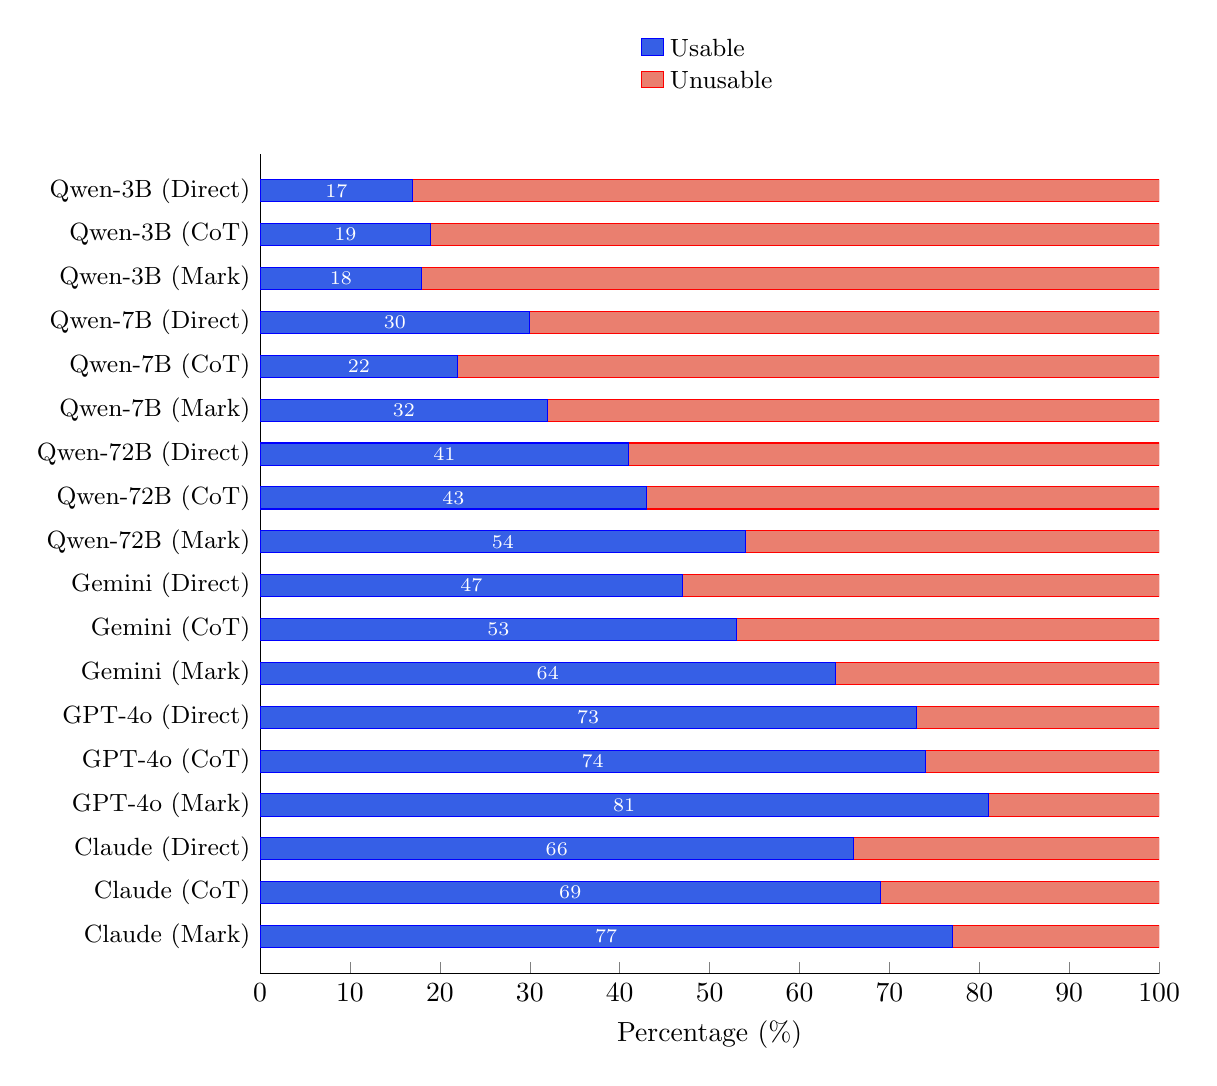
\begin{tikzpicture}
\begin{axis}[
  % --- Achsen-/Diagramm-Eigenschaften -------------------
  xbar stacked,                 % horizontale, gestapelte Balken
  xmin=0, xmax=100,             % 0–100 %
  width=13cm, height=12cm,      % Gesamtgröße
  bar width=8pt,                % Balkendicke
  enlarge y limits=0.05,        % etwas Luft oben/unten
  xlabel={Percentage (\%)},
  axis x line*=bottom,          % nur untere x-Achse
  axis y line*=left,            % nur linke y-Achse
  ytick=data,                   % ein Tick pro Kategorie
  y tick label style={font=\small},
  % --- Legende oben -------------------------------------
  legend style={
    at={(0.5,1.06)}, anchor=south, draw=none,
    legend cell align=left, font=\small
  },
  % --- Werte im Balken (nur im 1. Plot) -----------------
  nodes near coords,
  nodes near coords style={
    font=\scriptsize\bfseries, text=white, anchor=center
  },
  every node near coord/.append style={
    /pgf/number format/.cd, fixed, precision=0,  % nur ganze %
    /tikz/.cd
  },
  % --- Kategorien (y-Achse) in genau der Reihenfolge ----
  symbolic y coords={
    Claude (Mark), Claude (CoT), Claude (Direct),
    GPT-4o (Mark), GPT-4o (CoT), GPT-4o (Direct),
    Gemini (Mark), Gemini (CoT), Gemini (Direct),
    Qwen-72B (Mark), Qwen-72B (CoT), Qwen-72B (Direct),
    Qwen-7B (Mark), Qwen-7B (CoT), Qwen-7B (Direct),
    Qwen-3B (Mark), Qwen-3B (CoT), Qwen-3B (Direct)
  }
]
% ---------- 1. Plot: Usable (blau) + Prozentzahlen -------
% ---------- 1. Plot: Usable -----------------------------
\addplot+[xbar,fill=usable] coordinates {
  (77,{Claude (Mark)})   (69,{Claude (CoT)})   (66,{Claude (Direct)})
  (81,{GPT-4o (Mark)})   (74,{GPT-4o (CoT)})   (73,{GPT-4o (Direct)})
  (64,{Gemini (Mark)})   (53,{Gemini (CoT)})   (47,{Gemini (Direct)})
  (54,{Qwen-72B (Mark)}) (43,{Qwen-72B (CoT)}) (41,{Qwen-72B (Direct)})
  (32,{Qwen-7B (Mark)})  (22,{Qwen-7B (CoT)})  (30,{Qwen-7B (Direct)})
  (18,{Qwen-3B (Mark)})  (19,{Qwen-3B (CoT)})  (17,{Qwen-3B (Direct)})
};

% ---------- 2. Plot: Unusable ---------------------------
\addplot+[xbar,fill=unusable,nodes near coords={}] coordinates {
  (23,{Claude (Mark)})   (31,{Claude (CoT)})   (34,{Claude (Direct)})
  (19,{GPT-4o (Mark)})   (26,{GPT-4o (CoT)})   (27,{GPT-4o (Direct)})
  (36,{Gemini (Mark)})   (47,{Gemini (CoT)})   (53,{Gemini (Direct)})
  (46,{Qwen-72B (Mark)}) (57,{Qwen-72B (CoT)}) (59,{Qwen-72B (Direct)})
  (68,{Qwen-7B (Mark)})  (78,{Qwen-7B (CoT)})  (70,{Qwen-7B (Direct)})
  (82,{Qwen-3B (Mark)})  (81,{Qwen-3B (CoT)})  (83,{Qwen-3B (Direct)})
};

\legend{Usable, Unusable}
\end{axis}
\end{tikzpicture}
